% 02_previous_work_first.tex

Most work in deep learning for CSI estimation focuses on different neural network architectures, training frameworks, or hyperparameter tuning. However, the normalization used in these works is typically the same; the extrema (i.e., the minimum and the maximum) of the dataset are used to perform minmax scaling on the entire dataset, 

\begin{align*}
	H^n_{\text{minmax}}(i,j) &= \frac{H^n(i,j)-H_{\text{min}}}{H_{\text{max}}-H_{\text{min}}}
\end{align*}
for $n \in [1,\dots,N]$ given a dataset of $N$ samples and $i,j$ indexing the rows/columns of the CSI matrices. The resulting samples are cast to the range $[0,1]$.

For image data, minmax normalization results in each image's color channels scaled to the range $[0,1]$. The resulting distribution for each color channel is typically satisfactory for image tasks, as the variance is not much smaller than the range of the normalized data (see Fig.~\ref{fig:imagenet_dist}).

However, for CSI matrices, minmax normalization is applied to the real and imaginary channels of each element. For typical channel models and parameters, the distribution of channel elements (see Fig.~\ref{fig:cost_indoor_dist}) tends to have much lower variance than that of ImageNet. This smaller variance can be explained by the difference in the datasets' ranges -- while the channels in image data (e.g., ImageNet) assume integer values between $[0,255]$, the channels in CSI data (e.g., COST2100) assume floating point values smaller than $10^{-3}$.

\begin{figure}[htb]
	\centering
	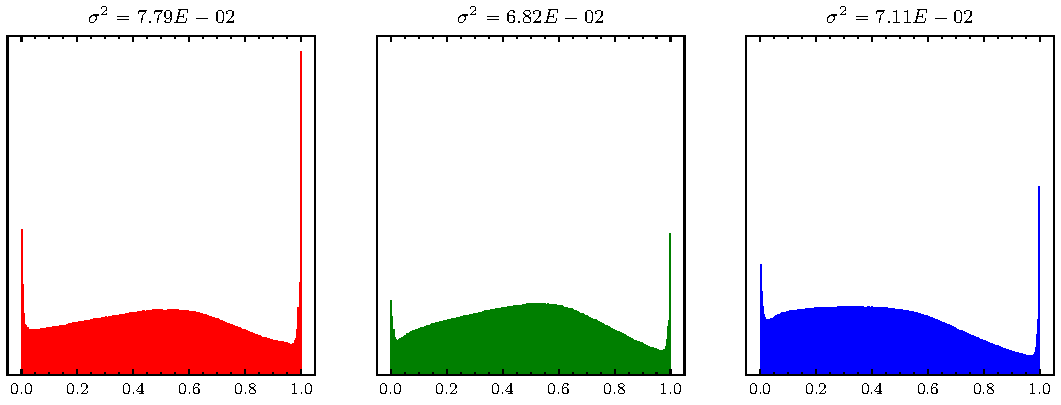
\includegraphics[width=.9\textwidth]{imagenet_rgb_dist.pdf}
	\medskip
	\caption{Distribution and variance of ImageNet color channels ($N=50000$) images.}
	\label{fig:imagenet_dist}
\end{figure}

\begin{figure}[htb]
	\centering
	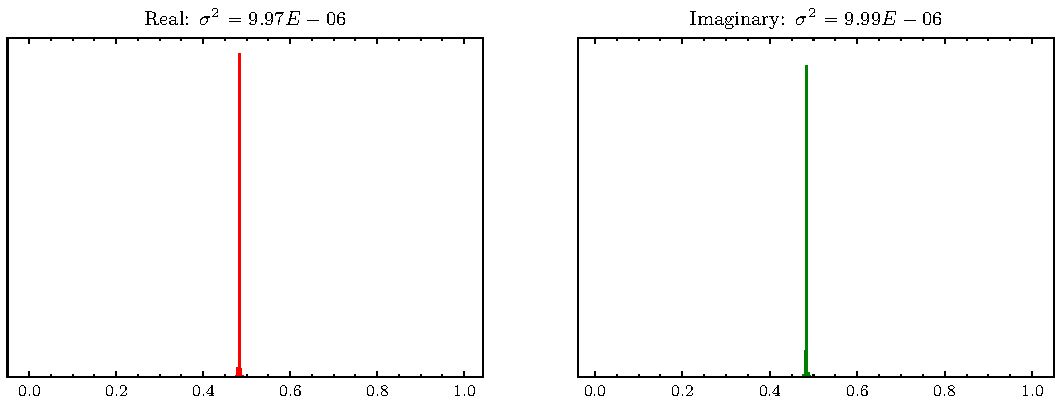
\includegraphics[width=.9\textwidth]{cost2100_indoor_dist.pdf}
	\medskip
	\caption{Distribution and variance of COST2100 real/imaginary channels ($N=99000$) images.}
	\label{fig:cost_indoor_dist}
\end{figure}

\blindtext

\subsection{Related Work}

Several works have investigated normalization techniques for deep learning such as batch normalization \cite{ref:ioffe2015batch}, instance normalization \cite{ref:huang2017instance}, layer normalization \cite{ref:ba2016layer}, and group normalization \cite{ref:wu2018group}. These normalization techniques scale the outputs of latent layers in neural networks, which helps to solve the problem of covariate shift \cite{ref:ioffe2015batch} where the mean and variance of changes between subsequent layers of the network.

Other works have studied normalization of the network's inputs. A number of works have investigated adaptive normalization techniques for time series estimation tasks \cite{ref:ogasawara2010adpative, ref:nayak2014impact, ref:shao2015self}. In \cite{ref:passalis2019dain}, the authors proposed a trainable input network which learns to shift, scale, and filter the unnormalized data while training the target network for a time series prediction task.

\blindtext
\blindtext

\subsection{Methods}



\blindtext

\subsubsection{Notation}

For an example of a table, see Table~\ref{table:notation}.

\begin{table}[htb]
	%	\small
	\caption{Notations}
	\label{table:notation}
	\centering
	\begin{tabular}[]{c|l}
		\toprule
		Variable & Definition \\
		\midrule
		$M$ & Number of input hydrological variables denoted in Fig.~\ref{fig:ann_inputs}\\
		\hline
		$N$ & Number of data samples, or days, in dataset \\
		\hline
		$T$ & Number of days' data used for estimation \\
		\hline
		$T_r$ & Dimension of data after pre-processing\\
		\hline
		$z_{n}$ & Time series used for estimating salinity level on day $n$, size is ${\rm I\!R}^{M\times T}$ \\
		\hline
		$x_{n}$ & Pre-processed time series with size ${\rm I\!R}^{M\times T_r}$ for day $n$\\
		\hline
		$f$ & A convolutional filter with size ${\rm I\!R}^{M \times T \times T_r}$ \\
		\hline
		$y_{n}$ & ANN-estimated salinity level for one or more locations on day $n$ \\
		\bottomrule
	\end{tabular}
\end{table}

% \begin{figure}[htb]
% 	\centering
% 	\includegraphics[width=.7\textwidth]{math_pipeline.png}
% 	\medskip
% 	\caption{Pipeline for ANNs in \cite{jayasundara2020artificial} with mathematical notations}
% 	\label{fig:math_pipeline}
% \end{figure}

\subsubsection{Spherical Normalization}
\label{sect:sph_norm_method}
Rather than apply minmax normalization, which is adversely impacted by outliers, we propose spherical normalization. Before describing spherical normalization in detail, consider z-score normalization. Given a random variable, $x$, with mean $\mu x$ and standard deviation $\mu$. The z-score normalized version of this random variable is given as
\begin{align}
	z &= \frac{x - \mu}{\sigma^2}. \label{eq:zscore}
\end{align}
Assuming $x$ is normally distributed, the resulting random variable, $z$, is a standard normal distribution such that $z \sim \mathcal N(0,1)$. Inspired by $z$-score normalization, we seek a normalization scheme which adjusts the range of each channel sample. Under spherical normalization, each sample in the dataset is scaled by its power. Denote the $k$-th downlink CSI matrix of the dataset as $\mathbf H_d^k$. The spherically normalized version of the downlink CSI is given as
% TODO: Does this make sense? "For CSI matrices, we could choose to scale each element by it's mean and by the inverse covariance matrix."
\begin{align}
	\mathbf{\check H}_d^k &= \frac{\mathbf H_d^k}{\|\mathbf H_d^k\|_2}. \label{eq:sph-intro}
\end{align}
Observe that (\ref{eq:sph-intro}) is similar to (\ref{eq:zscore}) without the mean shift in the numerator and with the power term of each CSI sample rather than the variance of the entire distribution. After applying (\ref{eq:sph-intro}) to each sample, minmax scaling is applied to the entire dataset. The resulting dataset under spherical normalization can exhibit a larger variance than the same dataset under minmax scaling, as is demonstrated in Fig.~\ref{fig:cost_indoor_sph_dist}. 
\begin{figure}[htb]
	\centering
	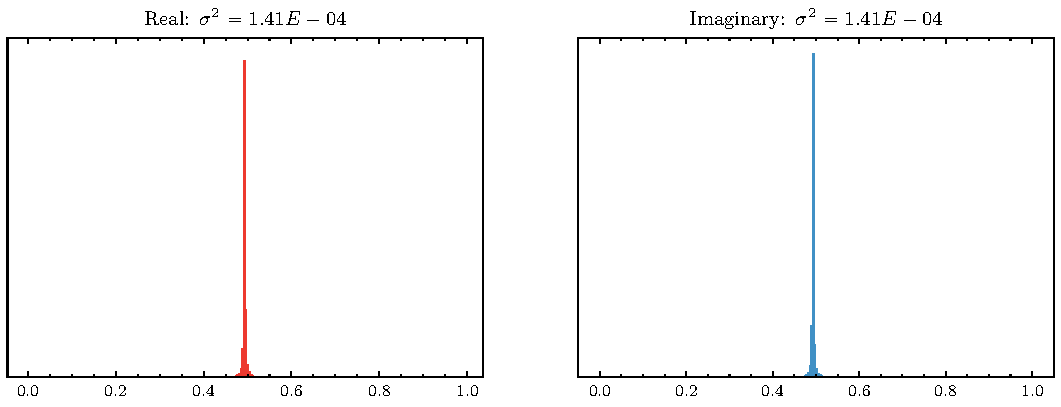
\includegraphics[width=.9\textwidth]{cost2100_indoor_sph_dist.pdf}
	\medskip
	\caption{Distribution and variance of COST2100 real/imaginary channels under spherical normalization ($N=99000$) images.}
	\label{fig:cost_indoor_sph_dist}
\end{figure}

\blindtext
\blindtext

\subsubsection{Methods Subsection \#2}
\label{sect:methods_sub2}

\blindtext

\begin{equation}
x_{n,i}^{(m)} = \sum_{j=1}^{T}z_{n-j+1}^{(m)}\times f_{j,i}^{(m)},
\label{eq:conv}
\end{equation}

\blindtext
